\documentclass[a4paper, 14pt]{extarticle}

\usepackage[T2A]{fontenc}
\usepackage{natbib}
\usepackage{graphicx}
\usepackage[english, russian]{babel}
\usepackage{fontspec}
\usepackage{amsmath}
\usepackage{amsfonts}
\usepackage{amssymb}
\usepackage{amsthm}
\usepackage{mathtools}
\usepackage{mathrsfs}
\usepackage{icomma}
\usepackage{fullpage}
\usepackage{ulem}
\usepackage{setspace}
\usepackage{listings}
\usepackage{indentfirst}
\usepackage[left=2cm,right=1.5cm,top=2cm,bottom=2cm]{geometry}
\usepackage{xcolor}
\usepackage{float}
\usepackage{csquotes}
\usepackage{hyperref}
\usepackage{graphics}



\definecolor{urlcolor}{HTML}{0000FF} % цвет гиперссылок
\definecolor{linkcolor}{HTML}{000000} % цвет гиперссылок
\hypersetup{pdfstartview=FitH, linkcolor=linkcolor, urlcolor=urlcolor, colorlinks=true}


\setmainfont{Times New Roman}
\setlength{\parindent}{5ex}
\setlength{\parskip}{1em}
\renewcommand{\baselinestretch}{1}

\graphicspath{{images/}}


\definecolor{buzzlightyear}{HTML}{8757A5}
\definecolor{grass}{HTML}{738D06}
\definecolor{literal}{HTML}{F18A2B}
\definecolor{commentcolor}{HTML}{8E908B}

\lstdefinestyle{habrstyle}{
    backgroundcolor=\color{white},
    commentstyle=\color{commentcolor},
    keywordstyle=\bfseries\color{buzzlightyear},
    numberstyle=\tiny\color{commentcolor},
    stringstyle=\color{grass},
    basicstyle=\ttfamily\footnotesize,
    breakatwhitespace=false,
    breaklines=true,
    captionpos=b,
    keepspaces=true,
    numbers=left,
    numbersep=5pt,
    showspaces=false,
    showstringspaces=false,
    showtabs=false,
    tabsize=4
}

\lstset{style=habrstyle}

\begin{document}
    % НАЧАЛО ТИТУЛЬНОГО ЛИСТА
    \begin{center}
        \begin{center}
            \hfill \break
            \normalsize{Санкт-Петербургский государственный политехнический}\\
            \normalsize{университет Петра Великого}\\
            \hfill \break
            \normalsize{\textbf{Высшая школа интеллектуальных систем и}}\\
            \normalsize{\textbf{суперкомпьютерных технологий}}\\
            \hfill \break
            \hfill \break
            \hfill \break
            \normalsize{Лабораторная работа}\\
            \hfill \break
            \normalsize{\LARGE Апериодические сигналы}\\
        \end{center}
        \hfill \break
        \hfill \break
        \hfill \break
        \hfill \break
        \hfill \break
        \hfill \break
        \hfill \break
        \hfill \break
        \hfill \break
        \hfill \break
        \begin{tabbing}
            Выполнил студент гр. 3530901/80201 \`И.С. Иванов\\
            \\
            Преподаватель: \`Н.В. Богач\\
        \end{tabbing}
        \hfill \break
        \hfill \break
        \hfill \break
        \hfill \break
        \begin{center}
            Санкт-Петербург\\
            2021
        \end{center}
        \thispagestyle{empty}
    \end{center}
    % КОНЕЦ ТИТУЛЬНОГО ЛИСТА

    % ОГЛАВЛЕНИЕ
    \newpage
    \tableofcontents

    % СПИСОК ИЛЛЮСТРАЦИЙ
    \newpage
    \listoffigures

    % СПИСОК ЛИСТИНГОВ
    \newpage
    \lstlistoflistings

    \newpage


    \section{Упражнение №1: Изучить примеры из chap03}
    \label{sec:1_study_examples}

    Для выполнения первого пункта необходимо изучить и выполнить примеры из файла chap02.ipynb.
    Также необходимо в примере с утечкой заменить окно Хэмминга одним из окон, представляемых Numpy.

    Запустим все примеры из этого файла.

    \begin{figure}[H]
        \centering
        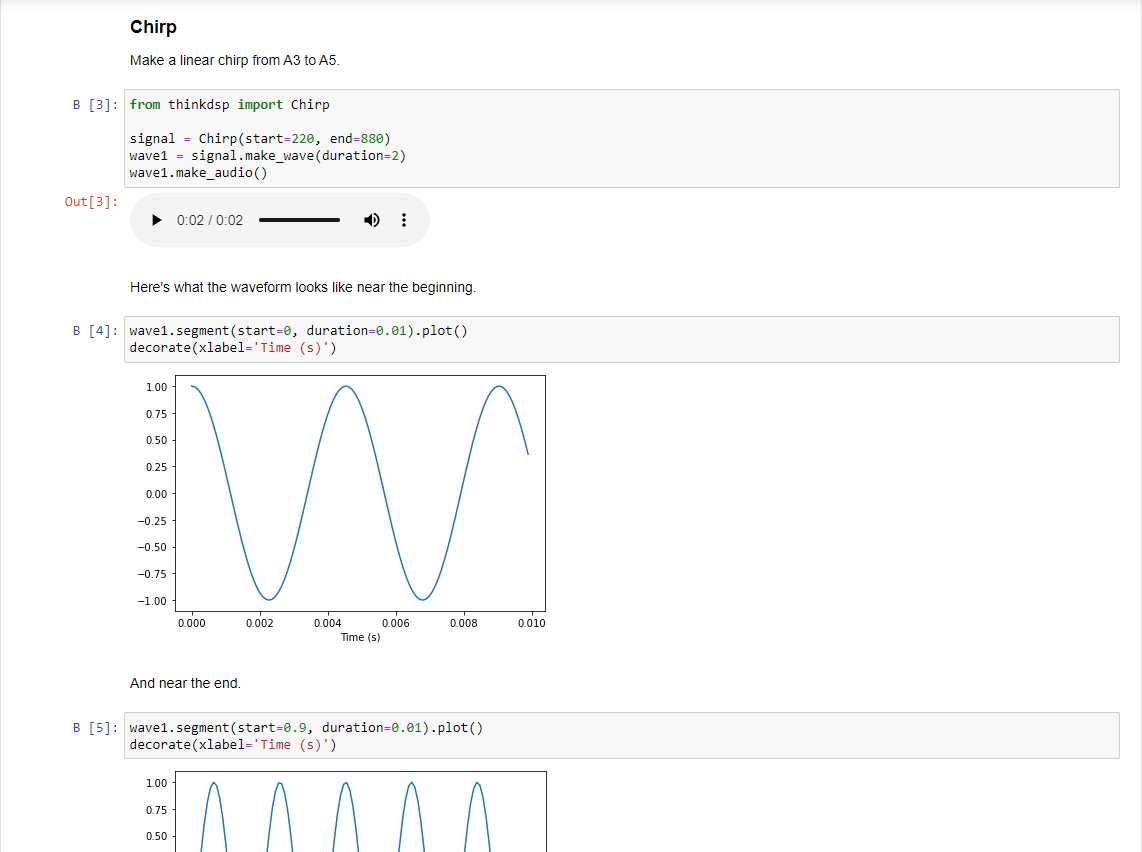
\includegraphics[width=0.8\linewidth]{check_work_1}
        \caption{Изучение и проверка примеров из файла (1)}
        \label{fig:check_it_works_1}
    \end{figure}

    \begin{figure}[H]
        \centering
        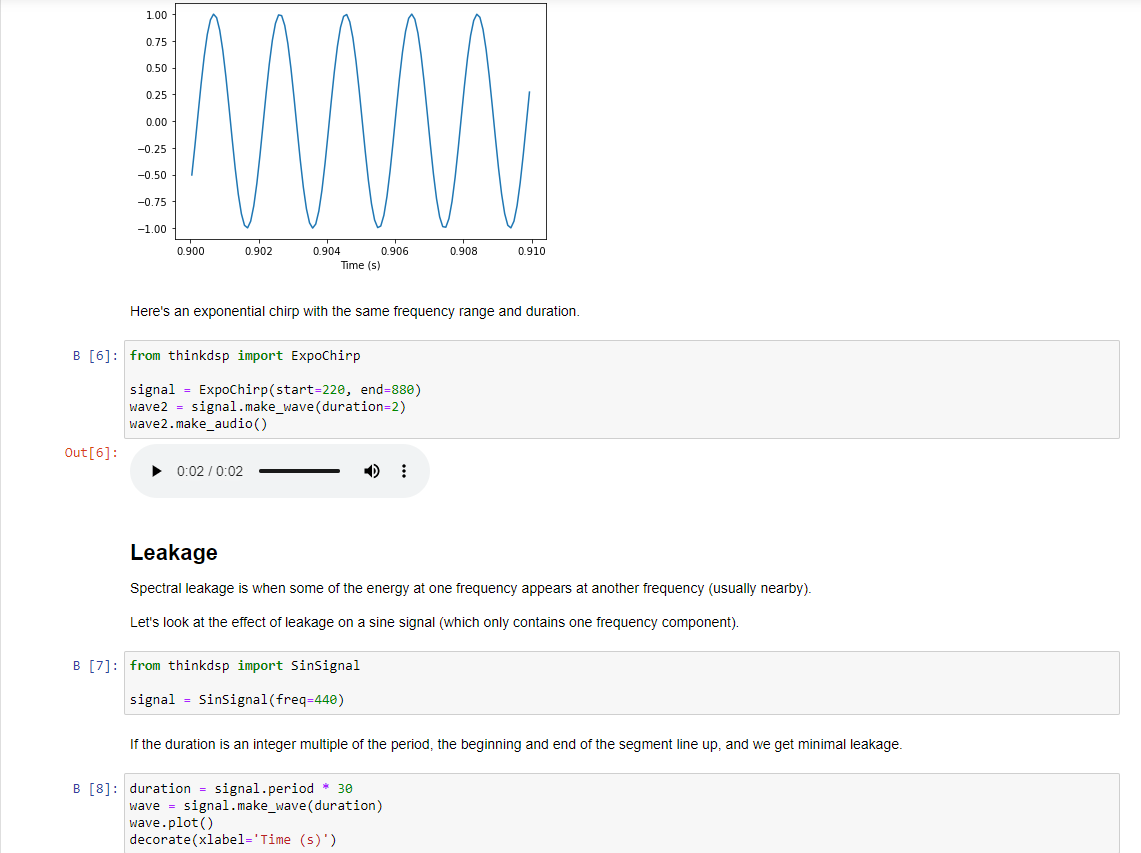
\includegraphics[width=0.8\linewidth]{check_work_2}
        \caption{Изучение и проверка примеров из файла (2)}
        \label{fig:check_it_works_2}
    \end{figure}

    Далее прогоним проверим окна предоставляемые NumPy и выведем все на график.

    \begin{lstlisting}[language=Python, caption= Проверка окон и вывод графика,label={lst:lstlisting}]
        for window_func in [np.bartlett, np.blackman, np.hamming, np.hanning]:
            wave = signal.make_wave(duration)
            wave.ys *= window_func(len(wave.ys))

            spectrum = wave.make_spectrum()
            spectrum.plot(high=880, label=window_func.__name__)
        decorate()
    \end{lstlisting}

    \begin{figure}[H]
        \centering
        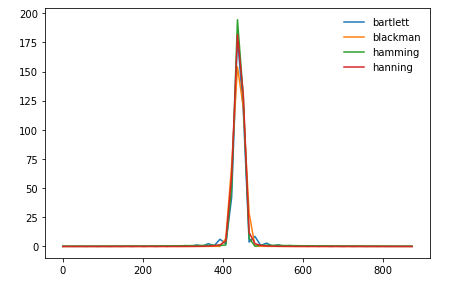
\includegraphics[width=0.8\linewidth]{compare_window}
        \caption{Сравнение окон из NumPy}
        \label{fig:compare_window}
    \end{figure}

    \newpage


    \section{Упражнение №2: SawtoothChirp}
    \label{sec:2_sawtooth_chirp}

    Во втором упражнении необходимо написать класс \texttt{SawtoothChirp}, который расширяет \texttt{Chirp} и переопределяет \texttt{evaluate} для генерации пилообразного сигнала c линейно увеличивающейся частотой.

    Подключение зависимостей и написание класса SawtoothSignal:

    \begin{lstlisting}[language=Python, caption= Класс SawtoothChirp, label={lst:sawtooth_chirp_code}]
        from thinkdsp import Chirp
        from thinkdsp import normalize, unbias

        PI2 = 2 * np.pi

        class SawtoothChirp(Chirp):
            def evaluate(self, ts):
                freqs = np.linspace(self.start, self.end, len(ts))
                dts = np.diff(ts, prepend=0)
                dphis = PI2 * freqs * dts
                phases = np.cumsum(dphis)
                cycles = phases / PI2
                frac, _ = np.modf(cycles)
                ys = normalize(unbias(frac), self.amp)
                return ys
    \end{lstlisting}

    Проверим работу класса.
    Выведем график сигнала и послушаем получившийся wav:

    \begin{lstlisting}[language=Python, caption= Вывод графика и создание wav, label={lst:create_wav_plot}]
        signal = SawtoothChirp(start=220, end=880)
        wave = signal.make_wave(duration=1, framerate=4000)
        wave.apodize()
        wave.make_audio()
    \end{lstlisting}

    Выведем конец сигнала.

    \begin{figure}[H]
        \centering
        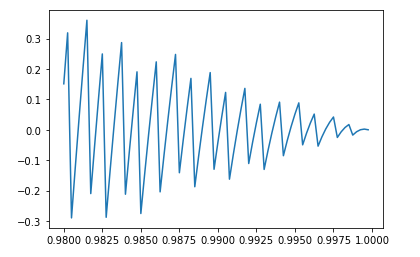
\includegraphics[width=0.8\linewidth]{sawtooth_chirp_signal_end}
        \caption{График конца сигнала}
        \label{fig:sawtooth_chirp_signal_end}
    \end{figure}

    Выведем спектрограмму:

    \begin{figure}[H]
        \centering
        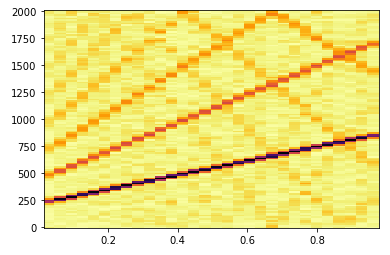
\includegraphics[width=0.8\linewidth]{sawtooth_chirp_sp}
        \caption{Спектрограмма сигнала}
        \label{fig:sawtooth_chirp_sp}
    \end{figure}

    По результатам выполнения данного упражнения был написан класс SawtoothChirp, генерирующий пилообразный сигнал с линейно увеличивающейся частотой.
    Класс был проверен созданием и прослушиванием аудио и изучением графика и спектрограммы.

    \newpage


    \section{Упражнение №3: Пилообразный сигнал (от 2500 Гц до 3000 Гц)}
    \label{sec:3_sawtooth_signal_hz}

    В третьем упражнении нам необходимо создать пилообразный chirp, меняющийся от 2500 до 3000 Гц, и на его основе сгенерировать сигнал длительностью 1с и framerate = 20 кГц.

    Создадим пилообразного сигнала и прослушаем его:

    \begin{lstlisting}[language=Python, caption= Создание сигнала и создание аудио, label={lst:make_sawtooth_hz}]
        signal = SawtoothChirp(start=2500, end=3000)
        wave = signal.make_wave(duration=1, framerate=20000)
        wave.make_audio()
    \end{lstlisting}

    Посмотри на его спектр.

    \begin{figure}[H]
        \centering
        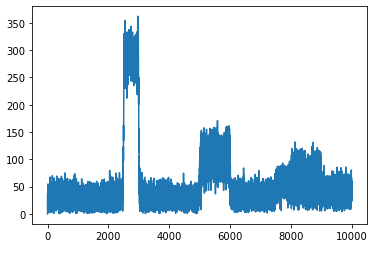
\includegraphics[width=0.8\linewidth]{sawtooth_hz_spectrum}
        \caption{Спектр нашего пилообразного сигнала}
        \label{fig:sawtooth_hz_spectrum}
    \end{figure}

    По результатам выполнения данного упражнения, сравнивая два сигнала, можно сделать вывод, что сигнал богат частотами.
    Аудио сигнала режет слух.

    \newpage


    \section{Упражнение №4: Глиссандо}
    \label{sec:4_glist}

    В четвертом упражнении необходимо скачать звук глиссандо и вывести спектрограмму.
    Звук был взят отсюда \href{https://archive.org/details/rhapblue11924}{https://archive.org/details/rhapblue11924}.

    Загрузка звука и выделение фрагмента:

    \begin{lstlisting}[language=Python, caption= Загрузка звука и выделения фрагмента, label={lst:load_wav_segment}]
        wave = read_wave('Sounds/rhapblue11924.wav').segment(start=7.75, duration=1.5)
        wave.make_audio()
    \end{lstlisting}

    Вывод спектрограммы.

    \begin{lstlisting}[language=Python, caption= Создание и вывод на экран треугольного сигнала, label={lst:print_spectrogram}]
        wave.make_spectrogram(512).plot(high=5000)
    \end{lstlisting}

    \begin{figure}[H]
        \centering
        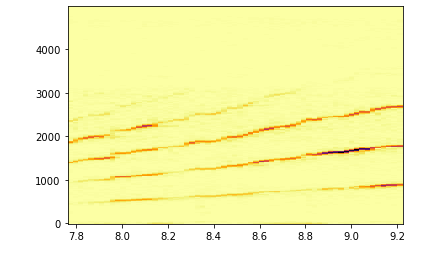
\includegraphics[width=0.8\linewidth]{glist_spectrogram}
        \caption{Спектрограмма глиссандо}
        \label{fig:glist_spectrogram}
    \end{figure}

    \newpage


    \section{Упражнение №5: TromboneGliss}
    \label{sec:5_trombone_gliss}

    В пятом упражнении необходимо написать класс \texttt{TromboneGliss}, расширяющий \texttt{Chirp} и преоставляющий \texttt{evaluate}.
    Создать сигнал, имитирующий глиссандо на тромбоне от C3 до F3 и обратно до C3.

    Создадим класс TromboneGliss:

    \begin{lstlisting}[language=Python, caption= Класс TromboneGliss, label={lst:trombone_gliss}]
        class TromboneGliss(Chirp):
            def evaluate(self, ts):
                l1, l2 = 1.0 / self.start, 1.0 / self.end
                lengths = np.linspace(l1, l2, len(ts))
                freqs = 1 / lengths

                dts = np.diff(ts, prepend=0)
                dphis = PI2 * freqs * dts
                phases = np.cumsum(dphis)
                ys = self.amp * np.cos(phases)
                return ys
    \end{lstlisting}

    Зададим требуемый сигнал

    \begin{lstlisting}[language=Python, caption={Создание сигнала, имитирующего глиссандо}, label={lst:make_signal_trombone_gliss}]
        low = 262
        high = 349
        signal = TromboneGliss(high, low)
        wave1 = signal.make_wave(duration=1)
        wave1.apodize()
        wave1.make_audio()

        signal = TromboneGliss(low, high)
        wave2 = signal.make_wave(duration=1)
        wave2.apodize()
        wave2.make_audio()

        wave = wave1 | wave2
        wave.make_audio()
    \end{lstlisting}

    Выведем спектрограмму.

    \begin{lstlisting}[language=Python, caption= Вывод спектрограммы сигнала, label={lst:plot_spectrogram}]
        sp = wave.make_spectrogram(1024)
        sp.plot(high=1000)
    \end{lstlisting}

    \begin{figure}[H]
        \centering
        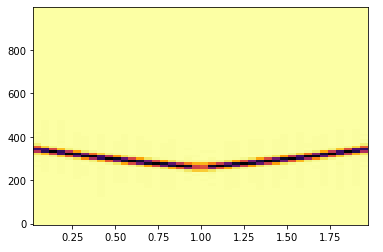
\includegraphics[width=0.8\linewidth]{trombone_gliss_spectrogram}
        \caption{Спектрограмма синтезированного глиссандо на тромбоне}
        \label{fig:trombone_gliss_spectrogram}
    \end{figure}


    \section{Упражнение №6: Анализ гласных}
    \label{sec:6_vowels}

    В шестом упражнении необходимо найти запись серии гласных звуков букв алфавита и построить их спектрограммы.

    Прочитаем файл со звуком и прошлушаем его:

    \begin{lstlisting}[language=Python, caption= Чтение и прослушивание аудио, label={lst:read_audio}]
        wave = read_wave('Sounds/87778__marcgascon7__vocals.wav')
        wave.make_audio()
    \end{lstlisting}

    Посмотрим на спектрограмму:

    \begin{lstlisting}[language=Python, caption= Спектр пилообразного сигнала, label={lst:vowels_spectrogram}]
        wave.make_spectrogram(1024).plot(high=1000)
    \end{lstlisting}

    \begin{figure}[H]
        \centering
        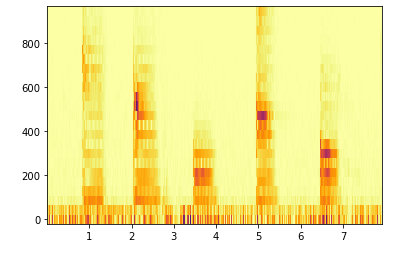
\includegraphics[width=0.8\linewidth]{vowels_spectrogram}
        \caption{Спектрограмма гласных}
        \label{fig:vowels_spectrogram}
    \end{figure}


    \section{Выводы}
    \label{sec:conclusions}

    В результате выполнения данной лабораторной работы мы изучили как надо работать с апериодическими сигналами, и что такое \texttt{chirp}.
    Также научились строить спектрограмму \texttt{chirp} и работать с \texttt{leakage}.
    Были реализованы классы для реализации пилообразного \texttt{chirp} и для имитации глиссадо на тромбоне.
    К этому всему были изучены спектрограммы гласных звуков.

\end{document}